% !TeX root = ../thuthesis-example.tex

\chapter{IoTDB 现有写入机制介绍与分析}
本章首先介绍 Apache IoTDB 目前已有的 \emph{insertRecords} 和 \emph{insertTablet} 接口,随后介绍 \emph{insertRecords} 写入接口执行的全部流程,包括客户端侧的数据封装、RPC 层的数据序列化与反序列化、存储引擎侧写入内存表以及最终持久化的过程。最后使用 IoT Benchmark 对 \emph{insertRecords} 接口进行性能测试和分析,找出目前 \emph{insertRecords} 接口性能不如预期的原因,为本文后续设计新 \emph{insertRecords} 写入机制提供参考。
\section{IoTDB 现有写入接口}
在 \ref{sec:chap1-sec1} 和 \ref{sec:chap1-sec2} 节中,我们简要介绍了 Apache IoTDB 现有的 \emph{insertRecords} 接口和 \emph{insertTablet} 接口,以及它们运行的整体流程。在本节中我们将进一步深入讨论 \emph{insertTablet} 和 \emph{insertRecords} 接口的设计以及两者在不同场景下的适用情况。

\subsection{Apache IoTDB 写入接口形式}
目前 IoTDB 主要提供了四种原生写入接口,分别是 \emph{insertRecord}、\emph{insertRecords}、\emph{insertTablet}、\emph{insertTablets}。这四种接口中 \emph{insertRecords}、\emph{insertTablet}、\emph{insertTablets} 都是批量化的写入接口,只有 \emph{insertRecord} 一次只写入一条记录。由于批量化写入可以将写入过程中的一些固定代价均摊到多个数据点上,可以减少写入总体代价\cite{bercken2001evaluation},因此 \emph{insertRecord} 的性能远不如其他三个接口,在生产环境中也几乎没有用户使用。以 IoTDB 的 Java SDK 为例,它们的接口定义如下:
\begin{lstlisting}[language=java,frame = trBL , firstnumber = last , escapeinside={(*@}{@*)}]
  void insertRecord(
      String deviceId,
      long time,
      List<String> measurements,
      List<TSDataType> types,
      List<Object> values
      )

  void insertRecords(
      List<String> deviceIds, 
      List<Long> times, 
      List<List<String>> measurementsList, 
      List<List<TSDataType>> typesList, 
      List<List<Object>> valuesList
      )

  void insertTablet(Tablet tablet)

  void insertTablets(Map<String, Tablet> tablets)
\end{lstlisting}
其中,Tablet 是一个数据结构,代表一个设备的一批数据,其结构如下:
\begin{lstlisting}[language=java,frame = trBL , firstnumber = last , escapeinside={(*@}{@*)}]
public class Tablet {
  public String deviceId;
  private List<MeasurementSchema> schemas;
  public long[] timestamps;
  public Object[] values;
  public int rowSize;
}
\end{lstlisting}
\emph{insertRecord} 和 \emph{insertRecords} 的参数含义则如表 \ref{tabular:insert-record-params} 和表 \ref{tabular:insert-records-params} 所示,\emph{Tablet} 的成员变量含义如表 \ref{tabular:class-tablet-param} 所示。
\begin{table}
  \centering
  \caption{insertRecord 参数说明}
  \begin{tabular}{lll}
    \toprule
    参数名 &  类型 & 描述 \\
    \midrule
    deviceId & String & 数据所属的设备 ID \\
    time & long & 数据的时间戳 \\
    measurements & List<String> & 每个数据点所属的时间序列 ID 组成的列表 \\
    types & List<TSDataType> & 每个数据点所对应的数据类型 \\
    values & List<Object> & 每个数据点的数据 \\
    \bottomrule
  \end{tabular}
  \label{tabular:insert-record-params}
\end{table}

\begin{table}
  \centering
  \caption{insertRecords 参数说明}
  \begin{tabular}{lll}
    \toprule
    参数名 &  类型 & 描述 \\
    \midrule
    deviceIds & List<String> & 每行记录所属的设备 ID 组成的列表 \\
     times & List<Long> & 每行记录的时间戳组成的列表 \\
    measurementsList & List<List<String> > & 每行记录的序列 ID 列表组成的列表 \\
    typesList & List<List<TSDataType> > & 每行记录数据类型列表组成的列表 \\
    valuesList & List<List<Object> > & 每行记录值列表组成的列表 \\
    \bottomrule
  \end{tabular}
  \label{tabular:insert-records-params}
\end{table}

\begin{table}
  \centering
  \caption{Tablet 类成员变量含义说明}
  \begin{tabular}{llp{6cm}}
    \toprule
    参数名 &  类型 & 描述 \\
    \midrule
    deviceId & String & 该 Tablet 所属的设备 ID \\
    schemas & List<MeasurementSchema> & 该 Tablet 中每个测点的元数据信息 \\
    timestmaps & long 类型数组 & 该 Tablet 中每一行数据的时间戳 \\
    values & Object 类型数组 & 该 Tablet 中每一个测点的数据,其中的每一个对象都代表一列数据 \\
    rowSize & int & 该 Tablet 中包含的数据行数\\
    \bottomrule
  \end{tabular}
  \label{tabular:class-tablet-param}
\end{table}

从接口形式上看,\emph{insertRecords}、\emph{insertTablet} 和 \emph{insertTablets} 其实都是在不同维度上进行批量化的写入接口:
\begin{itemize}
  \item \emph{insertRecords} 一次性可以写入多行数据,每一行数据都是任意一个设备在同一个时间戳下若干个测点的数据,不同行之间可以是不同的设备在不同时间戳下的数据。从这一点看,\emph{insertRecords} 是在多设备、多时间戳维度上进行批量化的写入接口。
  \item \emph{insertTablet} 一次写入一个 Tablet,每个 Tablet 只能包含一个设备在不同时间戳下的数据,不同设备的数据无法共享一个 Tablet。因此,\emph{insertTablet} 是对同一个设备在多时间戳维度上进行的批量化写入。
  \item \emph{insertTablets} 一次可以写入多个 Tablet,每个 Tablet 包含一个设备在不同时间戳下的数据。因此,\emph{insertTablets} 其实也是在多设备、多时间戳维度上进行批量化的写入接口。
\end{itemize}
\emph{insertRecords} 接口和 \emph{insertTablets} 接口在批量化的维度上是相同的,因此理论上使用 \emph{insertRecords} 接口的场景都可以使用 \emph{insertTablets},反之亦然。然而,由于 \emph{insertTablets} 接口要求用户先将需要写入的数据按照设备归类并封装成 Tablet 结构体,对于用户而言使用复杂度较高,\emph{insertRecords} 对数据形式的要求则更低,因此使用 \emph{insertRecords} 的用户数更多。
\subsection{不同写入接口的性能对比\label{sec:chap3-sec1-1}}
但是这两者在数据结构上有所不同。在 \emph{insertRecords} 中,属于同一个设备的数据可能会分布在不同的位置;在 \emph{insertTablets} 中,属于同一个设备的数据会被集中在同一个 Tablet 中。后一种模式能够在写入的后续处理流程中占有一些优势:数据在写入时首先进入内存表(MemTable)中,IoTDB 将同一个设备下的时间序列存储在内存表中的同一个块组(Chunk Group)中,如果同一个设备的数据都聚集在一起,那么就可以将它们一起写入到块组中,数据写入内存表的次数与 Tablet 的个数相同。而在 \emph{insertRecords} 的写入过程中,由于每一条 Record 都可能属于不同设备,因此只能一条一条 Record 地进行写入,写入内存表的次数与 Record 的数量相同,性能在某些情况下相比 \emph{insertTablets} 可能更低。

为了对比目前 \emph{insertRecords} 接口与 \emph{insertTablets} 的性能,笔者使用 IoTDB Benchmark\cite{liu2019benchmarking} 对 IoTDB 的 \emph{insertRecords} 和 \emph{insertTablets} 接口在不同的请求模式下进行测试。笔者固定单个写入请求的数据总行数为 400,调节单个请求中不同设备数,观察两种接口的性能变化\footnote{IoTDB 版本为 1.3.0,实验环境 CPU 为 I7-11700,DataNode 使用 28GB 内存,ConfigNode 2GB,硬盘为 HDD}。例如,如果一个请求中只有 1 个设备,那么一个请求中的 400 行都是该设备的数据;如果一个请求中有 10 个设备,那么请求中每个设备都各自有 40 行数据。图 \ref{fig:records-vs-tablets-throughput} 和图 \ref{fig:records-vs-tablets-latency} 分别展示了两种接口吞吐和延迟随设备数不同而出现的变化。

\begin{figure}
  \centering
  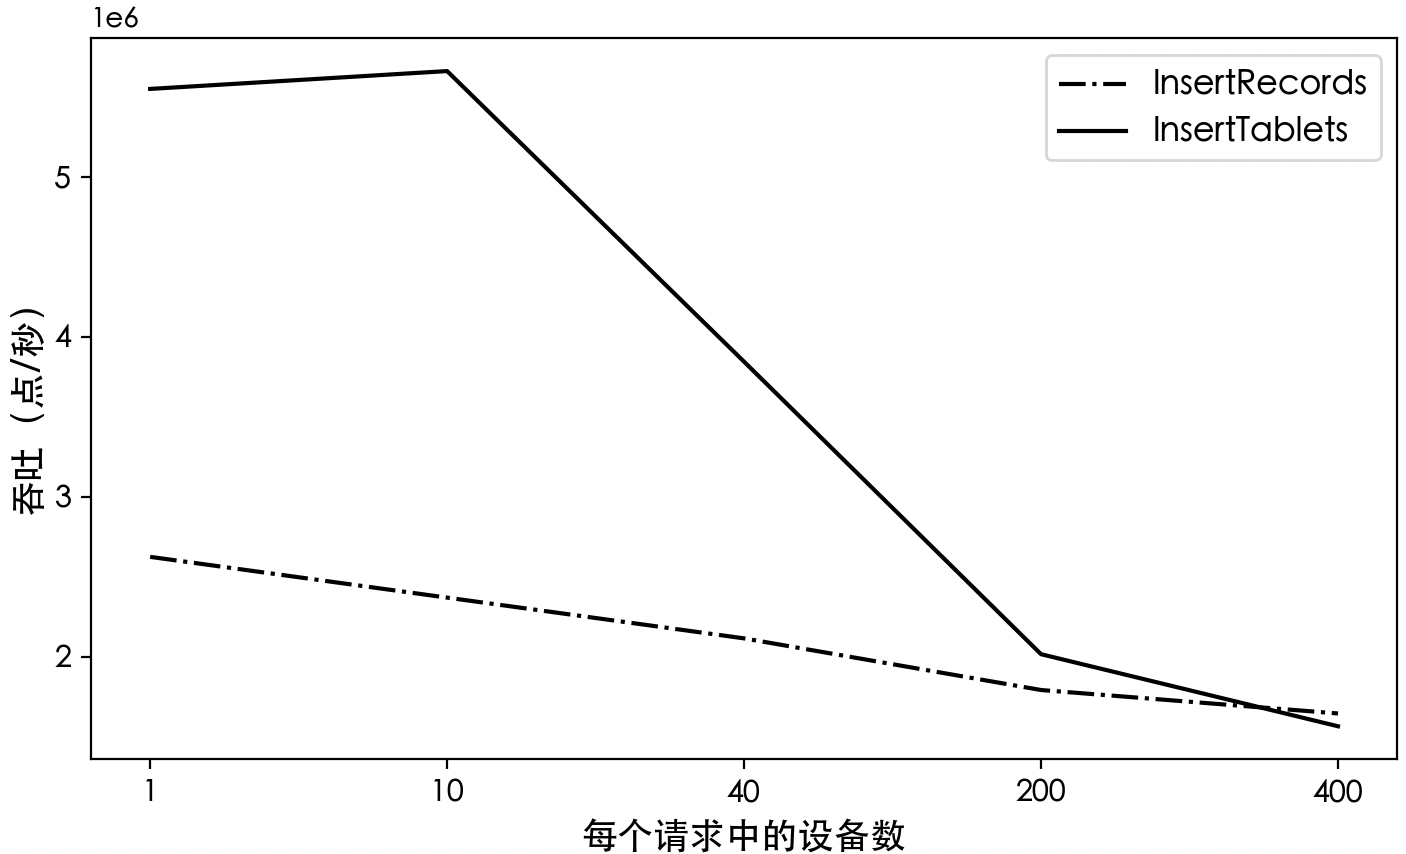
\includegraphics[width=\linewidth]{records-vs-tablets-throughput.png}
  \caption{一次写入请求中写入吞吐随设备数的变化}
  \label{fig:records-vs-tablets-throughput}
\end{figure}

\begin{figure}
  \centering
  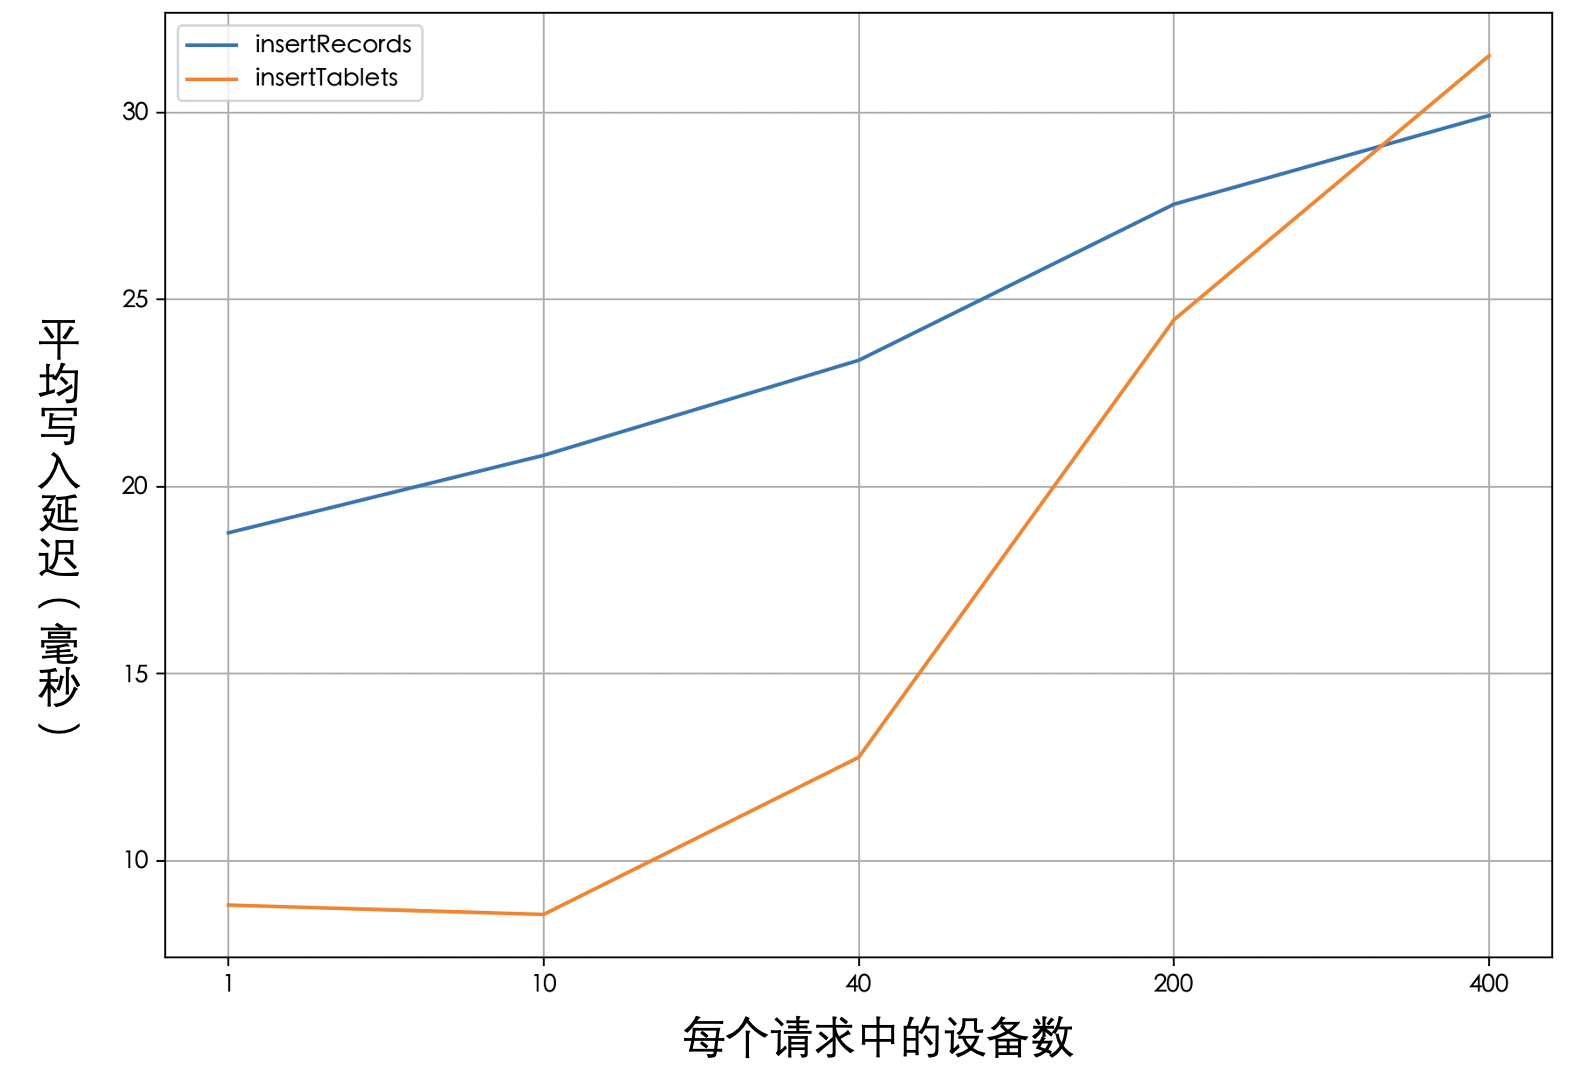
\includegraphics[width=\linewidth]{records-vs-tablets-latency.png}
  \caption{一次写入请求中写入延迟随设备数的变化}
  \label{fig:records-vs-tablets-latency}
\end{figure}

从实验结果中可以看出,当设备数小于 400,即每个设备都有超过 1 条数据时,\emph{insertTablets} 接口的性能要优于 \emph{insertRecords};当设备数等于 400 时,也就是每个设备在一次请求中都只有 1 条数据时,\emph{insertRecords} 接口要略微优于 \emph{insertTablets}。这个实验结论与上一节中对这两个接口的分析是一致的,使用 Tablet 写入可以利用同一设备的数据被提前聚集的特点进行批量化写入,实现较好的性能;而 \emph{insertRecords} 由于提前不知道同一设备数据的分布,只能一条一条地写入存储引擎,性能较差。当一个请求中每个设备都只有一条数据时,使用 \emph{insertTablets} 接口写入时每个 Tablet 都只有一行数据,此时其执行逻辑实际上和 \emph{insertRecords} 是差不多的。由于 \emph{insertRecords} 针对行式写入有一些优化,因此其性能略好于 \emph{insertTablets}。
\subsection{不同接口的使用场景}
\emph{insertRecords} 和 \emph{insertTablets} 接口在设备和时间两个维度进行了批量化,而 \emph{insertTablet} 接口则时间这个维度进行了批量化。不同批量化维度会导致不同接口的适用场景有所不同。

按照数据产生的频率进行划分,可以将时序数据写入的场景分为高频和中低频两种场景。在高频场景中,传感器的采样率很高,短时间内会产生大量时序数据,并且这些数据都属于同一个设备。例如在风力发电场景中风机上的传感器在某些情况下的采样频率可以达到 8KHz\cite{李天安2020apache},如果将一个风机建模为一个设备,并且假设传感器的采样频率一致,那么一个设备每秒钟就会产生 8000 行数据。在中低频场景中,传感器的采样频率较低,可能每隔几十秒传感器才会产生一个数据点。例如在长安汽车的车联网场景中,一辆汽车被建模为一个设备,汽车上的传感器每隔 30 秒才会进行一次采样,如果所有传感器的采样频率一致,那么一个设备每隔 30 秒才会产生一行数据。

数据产生频率的不同会导致这些场景适用不同接口。在高频场景中,由于一个设备的数据产生地非常快,使用 \emph{insertTablet} 或者 \emph{insertTablets} 接口可以充分利用数据按设备批量化的特点,将其快速写入到存储引擎中。如果使用 \emph{insertRecords} 接口,则无法利用每个设备下数据较多的特点,将数据一行一行地写入,导致最终性能不高。在低频场景中,数据间隔很久才会产生,如果使用 \emph{insertTablet} 或者 \emph{insertTablets} 接口就有两种选择:
\begin{enumerate}
  \item 为了提高写入性能,对数据进行缓存和积攒,等到 Tablet 的大小较大时才写入。但是这样会导致数据从产生到写入会经历非常长的时间。以长安汽车为例,一辆汽车被建模为一个设备,假如需要积攒到一个 Tablet 中有 100 行数据才写入,那么数据从产生到写入数据库的延迟为 50 分钟,在此期间其他应用无法从数据库中查询到这些数据,这是不可接受的。
  \item 为了及时写入数据,在每个 Tablet 较小时就进行写入。从上一节的实验结果中我们可以知道这样不仅无法发挥出 Tablet 写入的性能,对数据分 Tablet 进行组装还会对上层应用带来额外的复杂度。
\end{enumerate}
如果使用 \emph{insertRecords},可以令 Record 的数量积攒到一定程度以后一起发送给服务器进行写入,并且 \emph{insertRecords} 的接口形式更加直观,可以减轻用户侧的复杂度。因此,长安汽车在其业务中选择的就是 \emph{insertRecords} 接口进行数据写入。

但是,从 \ref{sec:chap3-sec1-1} 节中的实验结果不难发现,\emph{insertRecords} 接口虽然有着使用方便的优点,但是其性能与 \emph{insertTablets} 接口有一定的差距。因此,如果我们可以将 \emph{insertRecords} 写入接口的性能提升,那么对于用户而言既可以使用比较友好的接口,省去将数据归类为 Tablet 的繁琐过程,又可以获得不错的写入性能。所以,本文的研究重点是如何在保持 \emph{insertRecords} 接口不变的情况下,通过设计新的底层实现机制,实现高性能的 \emph{insertRecords} 写入。
\section{Apache IoTDB 中 \emph{insertRecords} 写入的实现}
在研究如何设计出新的 \emph{insertRecords} 写入实现机制之前,本文先介绍目前 Apache IoTDB 对 \emph{insertRecords} 写入机制的实现。从应用层调用 IoTDB SDK 提供的 \emph{insertRecords} 接口开始,写入会经历客户端侧的数据封装、RPC 层数据序列化与反序列化、存储引擎侧数据写入内存表以及内存表数据的持久化。下面将详细介绍这个过程。
\subsection{客户端侧的数据封装流程}
客户端在接收到用户传入的写入数据后,需要对数据进行校验、划分和封装,其操作如下:
\begin{itemize}
  \item \emph{insertRecords} 的每一个参数都是列表(List),在合法的语义下每个参数的长度应该相同,如果不同参数的列表长度不一致就需要停止写入并抛出错误。
  \item 经过校验之后,数据会进行分片。Apache IoTDB 是一个分布式的数据库,一个集群中可能存在多个数据节点。一条时间序列的数据会被切分成多片,分布在多个数据节点中\cite{wang2023apache}。用户通过接口传入的一批数据就可能需要写入不同的节点。为了更高效地写入,IoTDB 的客户端会缓存不同序列对应的数据节点地址,然后将传入的数据按照节点地址进行划分,写入同一个节点的数据集合成一个子请求。
  \item 每一个子请求都包含了用户写入的数据的若干行,包括这些行的设备 ID、时间序列 ID、数据类型、时间戳以及数据值。IoTDB 客户端在把数据交由 RPC 层进行传输前,会提前把数据类型以及数据值序列化为二进制数据。每一行序列化的格式都如图 \ref{fig:curr-line-serialize-format} 所示:首先序列化一个数据点的类型,然后是它的值,紧接着是下一个数据点的类型和值。一行数据序列化为一个字节流对象(ByteBuffer),一个请求中的多行数据序列化的结果是字节流对象的列表(List<ByteBuffer>),其中的每一个元素都代表了原来的一行数据。
\end{itemize}

\begin{figure}
  \centering
  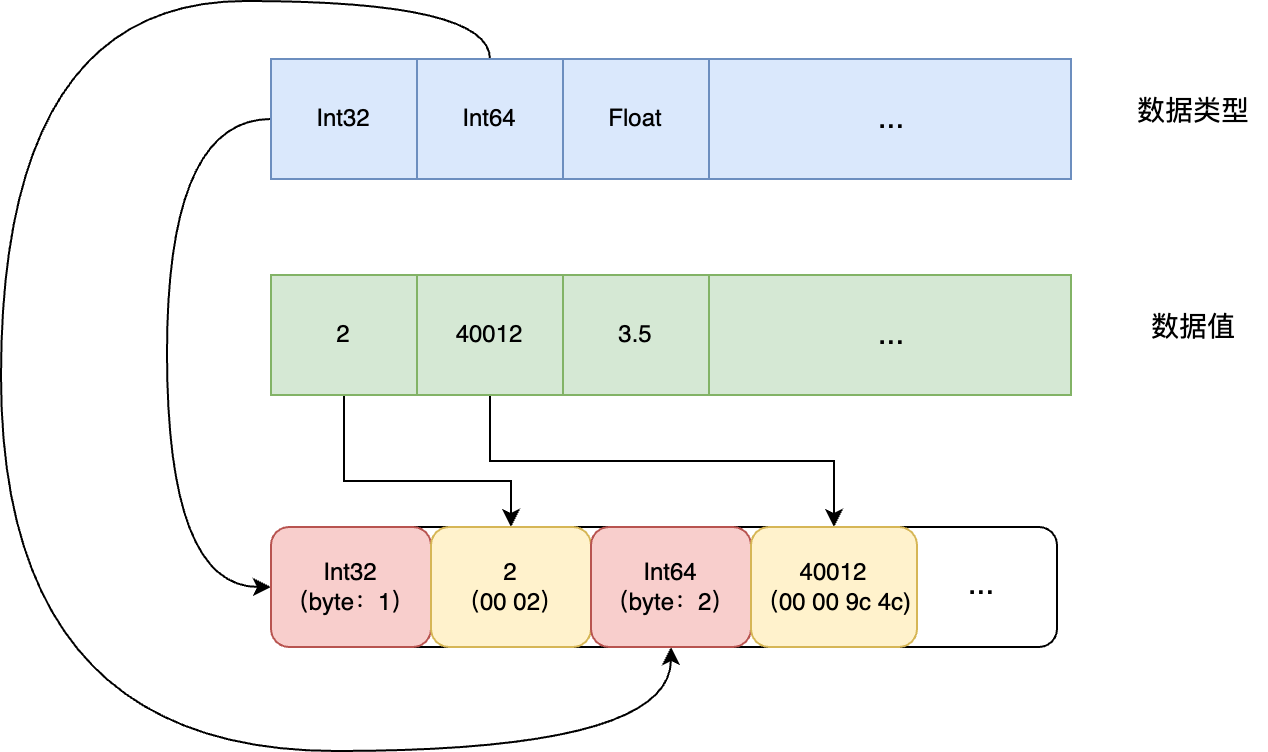
\includegraphics[width=\linewidth]{curr-data-serialize.png}
  \caption{一行数据序列化过程}
  \label{fig:curr-line-serialize-format}
\end{figure}

\subsection{RPC 层的数据序列化与反序列化流程}
\subsection{存储引擎侧数据写入内存表流程}
\subsection{存储引擎侧数据持久化流程}
\section{当前机制性能分析}
\section{本章小结}